\DiaryEntry{CORDIC (Coordinate Rotation Digital Computer)}{2024-05-13}{Maths}

The CORDIC is a simple and efficient algorithm to calculate trigonometric functions, hyperbolic functions, square roots, multiplications, divisions, and exponentials and logarithms with arbitrary base, typically converging with one digit (or bit) per iteration. 

\subsection{Rotation Mode}

In \emph{rotation mode}, CORDIC is used to calculate the sine and cosine of an angle given in radians.

To determine the sine or cosine for an angle $\beta$, the $y$ or $x$ coordinate of a point on the unit circle corresponding to the desired angle $\beta$ must be found (see Figure below).

Using CORDIC, one would start with the vector $\vbf_0$,

\bee
\vbf_{0} = \begin{pmatrix} 1 \\ 0 \end{pmatrix}
\eee

and proceed iteratively: In the first iteration, this vector is rotated $45$ degrees to get the vector $\vbf_{1}$. In the next iteration, the vector is rotated by a smaller angle in the direction which is closer to $\beta$ (in the example shown below, we rotate by counter-clockwise), yielding the vector $\vbf_2$. Successive iterations rotate the vector in one or the other direction by size-decreasing steps, until the desired angle has been achieved (in our example, the angle is sufficiently close to $\beta$ after the third iteration with the vector $\vbf_3$). We chose each step angle as $\gamma_{i}=\arctan(2^{-i})$ for $i=0,1,2,\ldots$.

% \input{images/2024-05-13-cordic_1}

\begin{figure}[H]
    \centering
    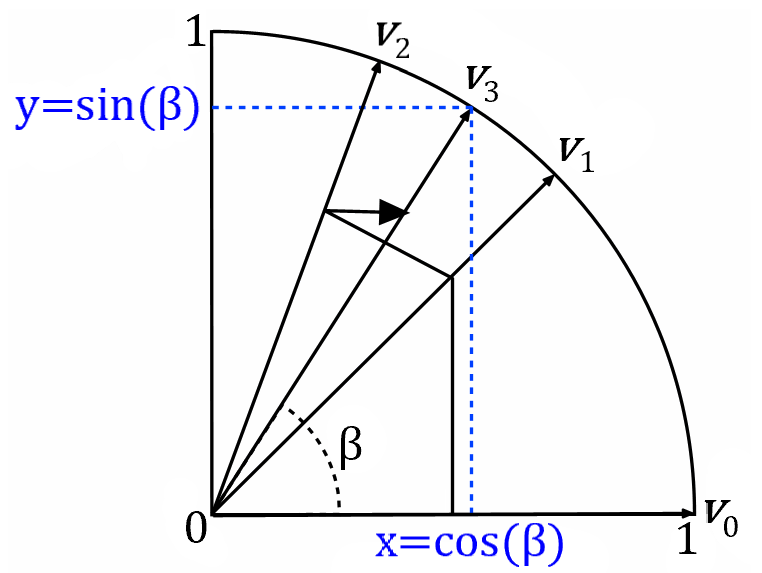
\includegraphics[scale=0.4]{images/2024-05-13-cordic_01.png}
\end{figure}

The vector after each rotation is denoted by $\vbf_{i+1}$ and it is obtained from $\vbf_i$ by multiplication with the rotation matrix $\Rbf$, 

\bee
\vbf_{i+1} = \Rbf \vbf_i \begin{pmatrix} \cos(\gamma_{i}) & -\sin(\gamma_{i}) \\ \sin(\gamma_{i}) & \cos(\gamma _{i}) \end{pmatrix} \vbf_i
\eee

Using the following two trigonometric identities:

\bee
\cos(\gamma_{i}) = \frac{1}{\sqrt {1+\tan ^{2}(\gamma_{i})}}
\eee

and

\bee
\sin(\gamma_{i}) =\frac{\tan(\gamma_{i})}{\sqrt {1+\tan ^{2}(\gamma_{i})}}
\eee

the rotation matrix becomes

\bee
\Rbf_{i} = \frac {1}{\sqrt {1+\tan ^{2}(\gamma _{i})}} \begin{pmatrix} 1 & -\tan(\gamma _{i}) \\ \tan(\gamma _{i}) & 1 \end{pmatrix}
\eee

and this yields for the rotated vector $\vbf_{i+1} = \Rbf_{i} \vbf_{i}$,

\bee
\begin{pmatrix} x_{i+1}\\ y_{i+1}\end{pmatrix} = \frac{1}{\sqrt {1+\tan^{2}(\gamma_{i})}} \begin{pmatrix} 1 & -\tan(\gamma_{i}) \\ \tan(\gamma_{i}) & 1 \end{pmatrix} \begin{pmatrix} x_{i} \\ y_{i} \end{pmatrix}
\eee

The final trick (mentioned above) is to choose the angle $\gamma_{i}$ for each iteration such that $\tan(\gamma_{i}) = \pm 2^{-i}$; this yields a series that converges to every possible output value. The multiplication with the tangent can therefore be replaced by a division by a power of two, which is efficiently done in digital computer hardware using a bit shift. The expression then becomes: 

\bee
\begin{pmatrix} x_{i+1}\\ y_{i+1}\end{pmatrix} = \frac {1}{\sqrt {1+2^{-2i}}} \begin{pmatrix} 1 & - \sigma_i 2^{-i} \\ \sigma_i 2^{-i} & 1 \end{pmatrix} \begin{pmatrix} x_{i} \\ y_{i} \end{pmatrix}
\eee

and $\sigma_{i} = \pm 1$ is used to determine the direction of the rotation: if the angle $\gamma _{i}$ is positive, then $\sigma _{i} = 1$, otherwise $\sigma _{i} = -1$.

The scaling factor is given by $\frac {1}{\sqrt {1+2^{-2i}}} = K_{i}$ and the factors can then be taken out of the iterative process and applied all at once afterwards with a scaling factor $K(n)$:

\bee    
K(n) = \prod_{i=0}^{n-1} K_{i} = \prod_{i=0}^{n-1} \frac {1}{\sqrt {1+2^{-2i}}}
\eee

which is calculated in advance and stored in a table.

The only task left is to determine whether the rotation should be clockwise or counterclockwise at each iteration (choosing the value of $\sigma$). This is done by keeping track of how much the angle was rotated at each iteration and subtracting that from the wanted angle; then in order to get closer to the wanted angle $\beta$, if $\beta_{n+1}$ is positive, the rotation is clockwise, otherwise it is negative and the rotation is counterclockwise:

\begin{align*}
    &\beta_{0} =\beta \\
    &\beta_{i+1} = \beta_{i} - \sigma_{i}\gamma_{i}, \quad \gamma_{i} = \arctan(2^{-i})
\end{align*}
    
The values of $\gamma_{n}$ must also be precomputed and stored.



%%% Local Variables:
%%% mode: latex
%%% TeX-master: "journal"
%%% End:
